\section{Aufbau}
\label{sec:Aufbau}
\begin{figure}
    \centering
    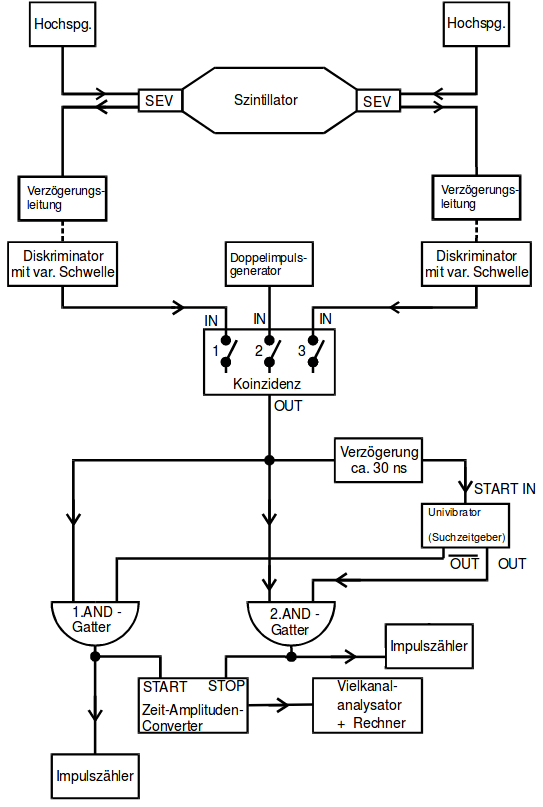
\includegraphics[width=\textwidth]{content/images/AufbauV01.png}
    \caption{Die Messschaltung zur Aufnahme von Individuallebensdauern kosmischer Myonen.}
    \label{fig:Aufbau}
    \end{figure}
%Bild muss noch angepasst werden(zweite verzögerungsleitung, zweiter impulszähler)

    Der Aufbau besteht aus zwei Teilen. Zunächst werden die Signale der auftretenden Myonen durch eine Schaltung geleitet, welche dazu dient Signale aufgrund von Störquellen herauszufiltern. Im Anschluss folgt eine Schaltung, welche die Zerfallszeiten misst und in für den Computer verwertbare Form umformt. Die in der Atmosphäre entstandenen Myonen gelangen zunächst in einen Szintillator. In diesem werden die zunächst relativistischen  Myonen abgebremst indem sie ihre kinetische Energie an die umliegenden Moleküle abgeben. Diese werden daraufhin in energetisch höhere Niveaus gehoben und sinken im Anschluss wieder in ihren Grundzustand. Ihre Energie geben sie in Form von Lichtquanten wieder ab. Diese liegen im sichtbaren Spektrum und im nahen UV Bereich. Da eine hohe zeitliche Genauigkeit benötigt wird, wird ein organischer Szintillator gewählt. Anschließend werden die Lichtquanten in zwei an beiden Seiten des Szintillators befestigten Photomultipliern in elektrische Signale umgewandelt und zur Verwertbarkeit um ca. um den Faktor $10^6$ verstärkt. Danach passieren die Impulse auf beiden Seiten eine Verzögerungsleitung und einen Diskriminator. In Letzterem werden die Signale einerseits von Störimpulsen niederer Spannung gefiltert und andererseits in eine einheitliche Form gebracht, mit welcher die nachfolgenden digitalen Bausteine arbeiten können. Die zweite Stufe der Filterung von Störquellen bildet eine Koinzidenzapperatur. Diese gibt nur ein Signal ab, falls an beiden Eingängen Impulse in ausreichend geringem zeitlichem Abstand auftreten. Da die störenden Untergundimpulse praktisch ausschließlich aufgrund von thermischen Elektronenemissionen im Anfangsbereich der Photomultiplier auftreten und dieser Prozess statistischer Natur ist, ist die Wahrscheinlichkeit das Störimpulse im benötigten Zeitraum auftreten vernachlässigbar klein. Die Lichtquanten bewegen sich hingegen schnell genug, sodass die Myonen zu zwei Impulsen im benötigten Zeitintervall führen.
    %unterer teil der schaltung
    Mit dem zweiten Teil der Schaltung lässt sich nun die Lebensdauer der Myonen bestimmen. Hierzu werden Myonen verwendet, welche bereits in der Atmosphäre ausreichend abgebremst wurden und im Szintillator nun zum Stillstand kommen. Da die vorherige Zeitdilatation nun aufhört zu wirken, kommt es zum Zerfall der Myonen. Die entstehenden Produkte besitzen wieder eine hohe kinetische Energie und werden ihrerseits im Szintillator abgebremst. Dies sorgt für einen zweiten Impuls kurz darauf. Der zeitliche Abstand beider Impulse liefert die inviduelle Lebensdauer des Myons. Die Schaltung ist nun wie folgt aufgebaut:
    Der erste Impuls läuft zu einem 1. AND-Gatter und zu einem 2. AND-Gatter. Da das 1. AND-Gatter über den $\bar{\text{OUT}}$  und das 2. AND-Gatter über den OUT-Zugang eines Univibrators verbunden ist, lässt nur das 1. AND-Gatter den Impuls durch, welcher in einen angeschlossenen Impulszähler sowie einen TAC gelangt. In letzterem startet Er die Zeitmessung. Nach ca. $\SI{30}{\nano\second}$ gelangt der Impuls auch in den Univibrator. Dieser klappt nun für eine eingestellte Zeit $T_s$ um. Gelangt in dieser Zeit ein zweiter Impuls in die Schaltung gelangt dieser durch das 2. AND-Gatter in den TAC und einen zweiten Impulszähler. Der TAC stoppt daraufhin die Messung und gibt einen proportional zur Zeit angestiegenen Strom an einen angeschlossenen Vielkanalanalysator mit 512 Kanälen weiter. In diesem werden die Impulse nach ihrer Höhe in einzelne Kanäle einsortiert und in jedem einzelnen gezählt. Die Messdaten können mit einem verbundenen Computer ausgelesen werden. Gelangt in der Zeit $T_\text{s}$ kein weiterer Impuls in die Schaltung, klappt der Univibrator wieder zurück und der nächste Impuls wird als neues Startsignal gewertet. Kommt es in der Zeit $T_\text{s}$ zur Abbremsung von zwei verschiedenen Myonen so werden diese als ein Zerfall gewertet. Dieser Untergrund lässt sich nicht herausfiltern und muss nachträglich bestimmt werden.          